% !TeX root = ../samplepaper.tex
\section{Results and Analysis}
\subsection{RQ1: Performance on TSP500}
两种GP控制器均改善了默认强度对照的求解质量。表\ref{tab:quality}中，\JS{}与\CT{}的平均reference gap分别为0.14759\%和0.15007\%，\Ueight{}为0.16942\%。对应改善为0.02183和0.01936个百分点，Holm校正后的$p$值分别为0.00015和0.00006，95\%区间均高于零（图\ref{fig:effects}）。这说明在相同底座与FE预算下，GP能够学到优于该静态配置的控制规则。

\begin{table}[tb]
\caption{冻结测试的平均reference gap（\%，越低越好）。每个规模128个实例、10个ACO seed；GP结果再平均3个GP seed。}
\label{tab:quality}
\centering\gentable{quality}
\end{table}

较强静态策略缩小了GP的优势。\Rsixteen{}与\Usixteen{}的gap为0.15163\%和0.15406\%，接近两种GP；这些配对差异的区间均跨越零，校正后未达到统计显著。相对\FACO{}的均值也有所降低，但没有得到显著差异。因此，现有结果支持GP超过MNE=8配置，尚不足以说明其稳定优于原生FACO适配版或MNE=16配置。下一节结合规则分析考察GP是否主要偏好较大扰动。

\begin{figure}[tb]
\centering\genfigure{effects}
\caption{相对各对照的gap改善及95\%分层配对bootstrap区间，单位为百分点。点在零线右侧表示GP更好；标签为“方法／对照”。星号仅标记TSP500九项Holm校正后$p<0.05$的比较；TSP1000为描述性区间。}
\label{fig:effects}
\end{figure}

本文用绝对百分点描述这些收益。例如，\JS{}相对\Ueight{}的逐求解平均路径长度改善约为0.02165\%；它与reference gap均值相对下降约12.9\%是不同量。后者表示剩余差距的缩小比例。

\subsection{RQ2: Learning Behaviour and Evolved Rules}
\paragraph{学习过程与选模.}
固定validation面板显示，两种表示随训练有小幅改善，但波动仍较大。图\ref{fig:curves}的下排使用训练结束后对每代冠军的quick-validation重评；按10代窗口平均，\JS{}从前10代的0.24250\%降至后10代的0.23166\%，\CT{}从0.24669\%降至0.22815\%。上排则以同代\Rsixteen{}为参照，消除部分训练面板难度变化。两种表示在TSP500测试中的差异为0.00247个百分点，区间跨零，未显示明确的表示优势。

\begin{figure}[tb]
\centering\genfigure{curves}
\caption{Training与quick validation。列分别为\JS{}和\CT{}；细线为三个GP seed，粗线为均值，均未平滑。上：训练冠军相对同代\Rsixteen{}的改善，正值更好；下：固定quick-validation面板重评的冠军gap，越低越好。下排在训练结束后计算，H1000，与最终选模的H5000 full validation不同。}
\label{fig:curves}
\end{figure}

Full validation所选的六个individual均不是末代训练冠军，只有两个是quick validation第一名。例如，\JS{}的seed 1103中，quick validation第四名在full validation达到0.12667\%，优于第一名的0.14551\%。这表明在当前设置下保留多个候选参与较长预算选模是有用的。两个validation阶段同时改变实例、ACO seed数和迭代预算，排名反转反映它们的综合影响。

末代种群仍保留结构和行为差异：每次运行有128个不同程序，在64个固定训练情境中产生100--115种动作向量；最大树高的中位数为4--5。不同fitness值有104--121个，说明终点评价可以区分多数individual。该训练信号仍是完整求解后的单个标量，多次在线决策及multi-tree的不同角色共同承担credit assignment。

\paragraph{从表达式理解控制偏好.}
六个选中individual包含5--35个节点。图\ref{fig:decoding}以两个seed 3313控制器展示规则如何得到动作；示例用于解释其结构与语义，全部六个individual见补充材料。\JS{}中最短的规则为
\begin{equation}
 f=\AQ\bigl(u,\AQ(\rho,d_R)\bigr).
 \label{eq:joint-rule}
\end{equation}
对固定区域，该式随MNE level $u$增大而增大，因此偏好MNE=16。当$\rho>0$时，较大的$d_R$使内层AQ减小、外层得分增大，规则倾向选择相邻端点更多落在区域外的起点集合。$\rho$接近零时，不同区域的分数差也趋小，实际选择可能由并列规则决定。

\begin{figure}[tb]
\centering
\begin{minipage}[c]{0.38\textwidth}\centering\small
\textbf{GP-J/3313}\par\medskip
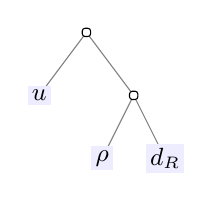
\begin{tikzpicture}[x=8mm,y=8mm,every node/.style={font=\small,inner sep=1.5pt}]
\draw[gray] (1.5,-1) -- (1,-2);
\draw[gray] (1.5,-1) -- (2,-2);
\draw[gray] (0.75,0) -- (0,-1);
\draw[gray] (0.75,0) -- (1.5,-1);
\node[fill=blue!7] at (0,-1) {$u$};
\node[fill=blue!7] at (1,-2) {$\rho$};
\node[fill=blue!7] at (2,-2) {$d_R$};
\node[draw,rounded corners=1pt,fill=white] at (1.5,-1) {$\AQ$};
\node[draw,rounded corners=1pt,fill=white] at (0.75,0) {$\AQ$};
\end{tikzpicture}
\par\medskip
\end{minipage}\hfill
\begin{minipage}[c]{0.59\textwidth}\centering\small
$\rho=0.00746447$，$u=1$\par
保留参考路径时：\par\smallskip
\begin{tabular}{cr}\toprule 区域$j$ & MNE16得分\\\midrule
0 & 0.999972165\\
1 & 0.999972165\\
2 & 0.999972999\\
3 & 0.999985993\\
\bottomrule\end{tabular}\par\smallskip
输出：$(r,j,\mathrm{MNE})=(0,3,16)$
\end{minipage}

\caption{选中规则与真实解码示例。左：\JS{}/3313的完整5节点树；右：\CT{}/3313的三棵树表达式及条件选择流程。下方给出两者各自在TSP500首个解释实例、ACO seed 17、第100迭代的分数；两条运行轨迹的状态不同。候选按编号排序，分数直接取自保存的CUDA回放。}
\label{fig:decoding}
\end{figure}

\CT{}/3313将三项决策分开，其区域规则为$p+\max(p,a_R\tau_R)$。同一决策状态中的$p$对各区域相同，因此区域偏好来自archive disagreement与pheromone strength的乘积：当乘积超过$p$时，该区域获得更高分。其强度规则为$u+(p+\rho)$，后两项是候选间的公共偏置，MNE排序由$u$决定。另两个\CT{}控制器的强度树在当前输入域内也偏好最大$u$。这些例子说明，表达式包含反馈terminal，并不意味着每项决策都随反馈改变。

\paragraph{观测动作与反馈响应.}
表达式中的强度偏好与已有回放一致。六个控制器在64个训练情境上共384次决策，以及两个规模的开发实例回放共144次决策，全部选择MNE=16。真实回放覆盖每规模2个实例和6个迭代位置；这些记录提供了策略行为的样本。

将停滞、回归率或工作量分别设为0或1后，MNE仍未变化，但部分区域与重启动作发生变化。图\ref{fig:decoding}中，\CT{}/3313的参考路径得分包含$w$与$s$，而强度树的反馈项是公共偏置，体现了反馈在不同角色中的不同作用。该诊断只改变固定状态下的输入，并未重新运行FACO，所以衡量的是动作敏感性。

完整测试的累计重启数进一步显示策略间差异。TSP500中，\JS{}三个控制器每5000迭代平均重启0、402.8、492.8次，\CT{}分别为433.8、231.4、726.4次。较高频率与当前接口缺少冷却期相符。结合静态MNE=16对照，后续需要通过完整求解实验分离区域选择与参考路径切换的收益；现有评分诊断尚不能回答这两部分是否改善了终点质量。

\subsection{RQ3: Transfer and Computational Cost}
TSP500训练所得策略在TSP1000上仍优于\Ueight{}的均值，但没有超过较强区域策略。\Rsixteen{}的reference gap为0.22825\%，低于\JS{}的0.25236\%和\CT{}的0.24563\%。两种GP相对它的改善分别为$-0.02411$和$-0.01738$个百分点，描述性95\%区间均位于零以下（图\ref{fig:effects}）。该结果表明，在当前测试族中，归一化特征和相同动作接口尚未使学习策略在更大规模上保持相对强静态对照的优势。

\begin{table}[tb]
\caption{计算成本。训练及监控／选模为每次GP运行的平均GPU任务分钟；测试列为TSP500每1280次求解的批处理摊销时间总和及每FE的平均LS移动评价数，GP再平均3个seed。静态策略不需要GP训练。}
\label{tab:maincost}
\centering\small\gentable{maincost}
\end{table}

\CT{}的训练成本高于\JS{}，而两者测试质量接近。表\ref{tab:maincost}中，平均训练GPU时间分别为393.21和283.72分钟，相差38.6\%；监控加选模约占训练的10.7\%和11.3\%。因此，当前conditional representation减少了每次决策的树求值次数，却没有降低完整训练成本。动作还会影响构造、local search和重启工作量，树求值次数只反映成本的一部分。

在两个测试规模上，GP的摊销GPU时间为\Ueight{}的约1.29--1.73倍，LS移动评价数为其约1.52--1.80倍。相同FE预算下，较高强度的搜索仍会消耗更多计算。已有同卡布局优化在四组种群样本上减少10.7\%--14.4\%的评价时间，细节列于补充材料。这里的GPU任务时间用于描述批处理成本，训练墙钟时间另列；不同服务器及CPU原生对照不用于计算直接加速倍数。
